Before diving into the core of the implementation, let's take an overview of the 
targetted system.

\begin{figure}[!htpb]
    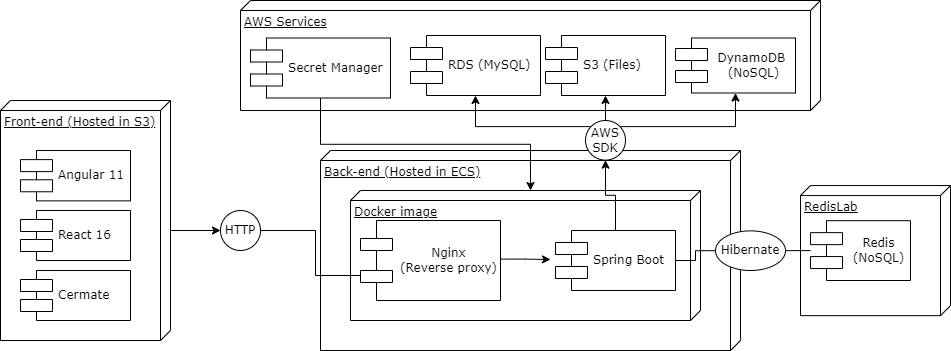
\includegraphics[width=\textwidth]{images/forecast}
    \caption{\footnotesize{Forecast component diagram}}
    \label{fig:forecast}
\end{figure}

As it's shown in \ref{fig:forecast} there are additional databases that are aimed to be
implemented mainly ones for archiving files as is the case of S3 and also archiving data
of the trucks and drivers that could be used for statistics and KPIs down the line thus
using DynamoDB\@.

With that in mind, the targetted systems database is divided into two main components:
    \begin{itemize}
        \item The archival database that is used to store the data of the trucks
            and drivers.
        \item The files database that is used to store the files that are uploaded
            by drivers and sites.
    \end{itemize}

The addition of a secrets manager, that is used to migrate the exposed secrets and
credentials, to assess the security of the system.

The removal or migration of the NodeJS backend code to a Java Backend, that could
manage the creation of a more uniform and aligned tech stack.

Also the transition to a more modern and trendy infrastructure that is based on 
containerization of the microservices and the use of Docker. Instead of the current
EC2 instances, which are not really required as the need to manual management and
configuration of modules within the containers could be automated within 
bash scripts.

There's the aim for the addition of CI/CD pipelines to the system, they could be
used to automate the deployment of the microservices and the creation of the
Docker images. Which in turn could ease up deployment of hotfixes, during the 
launch of new features and major updates.

We'll dive into the core of the implementation next.
